\newpage
\section{Serien- und Parallelschaltung von Zellen und Modulen}


\subsection{Serienschaltung von Solarzellen}
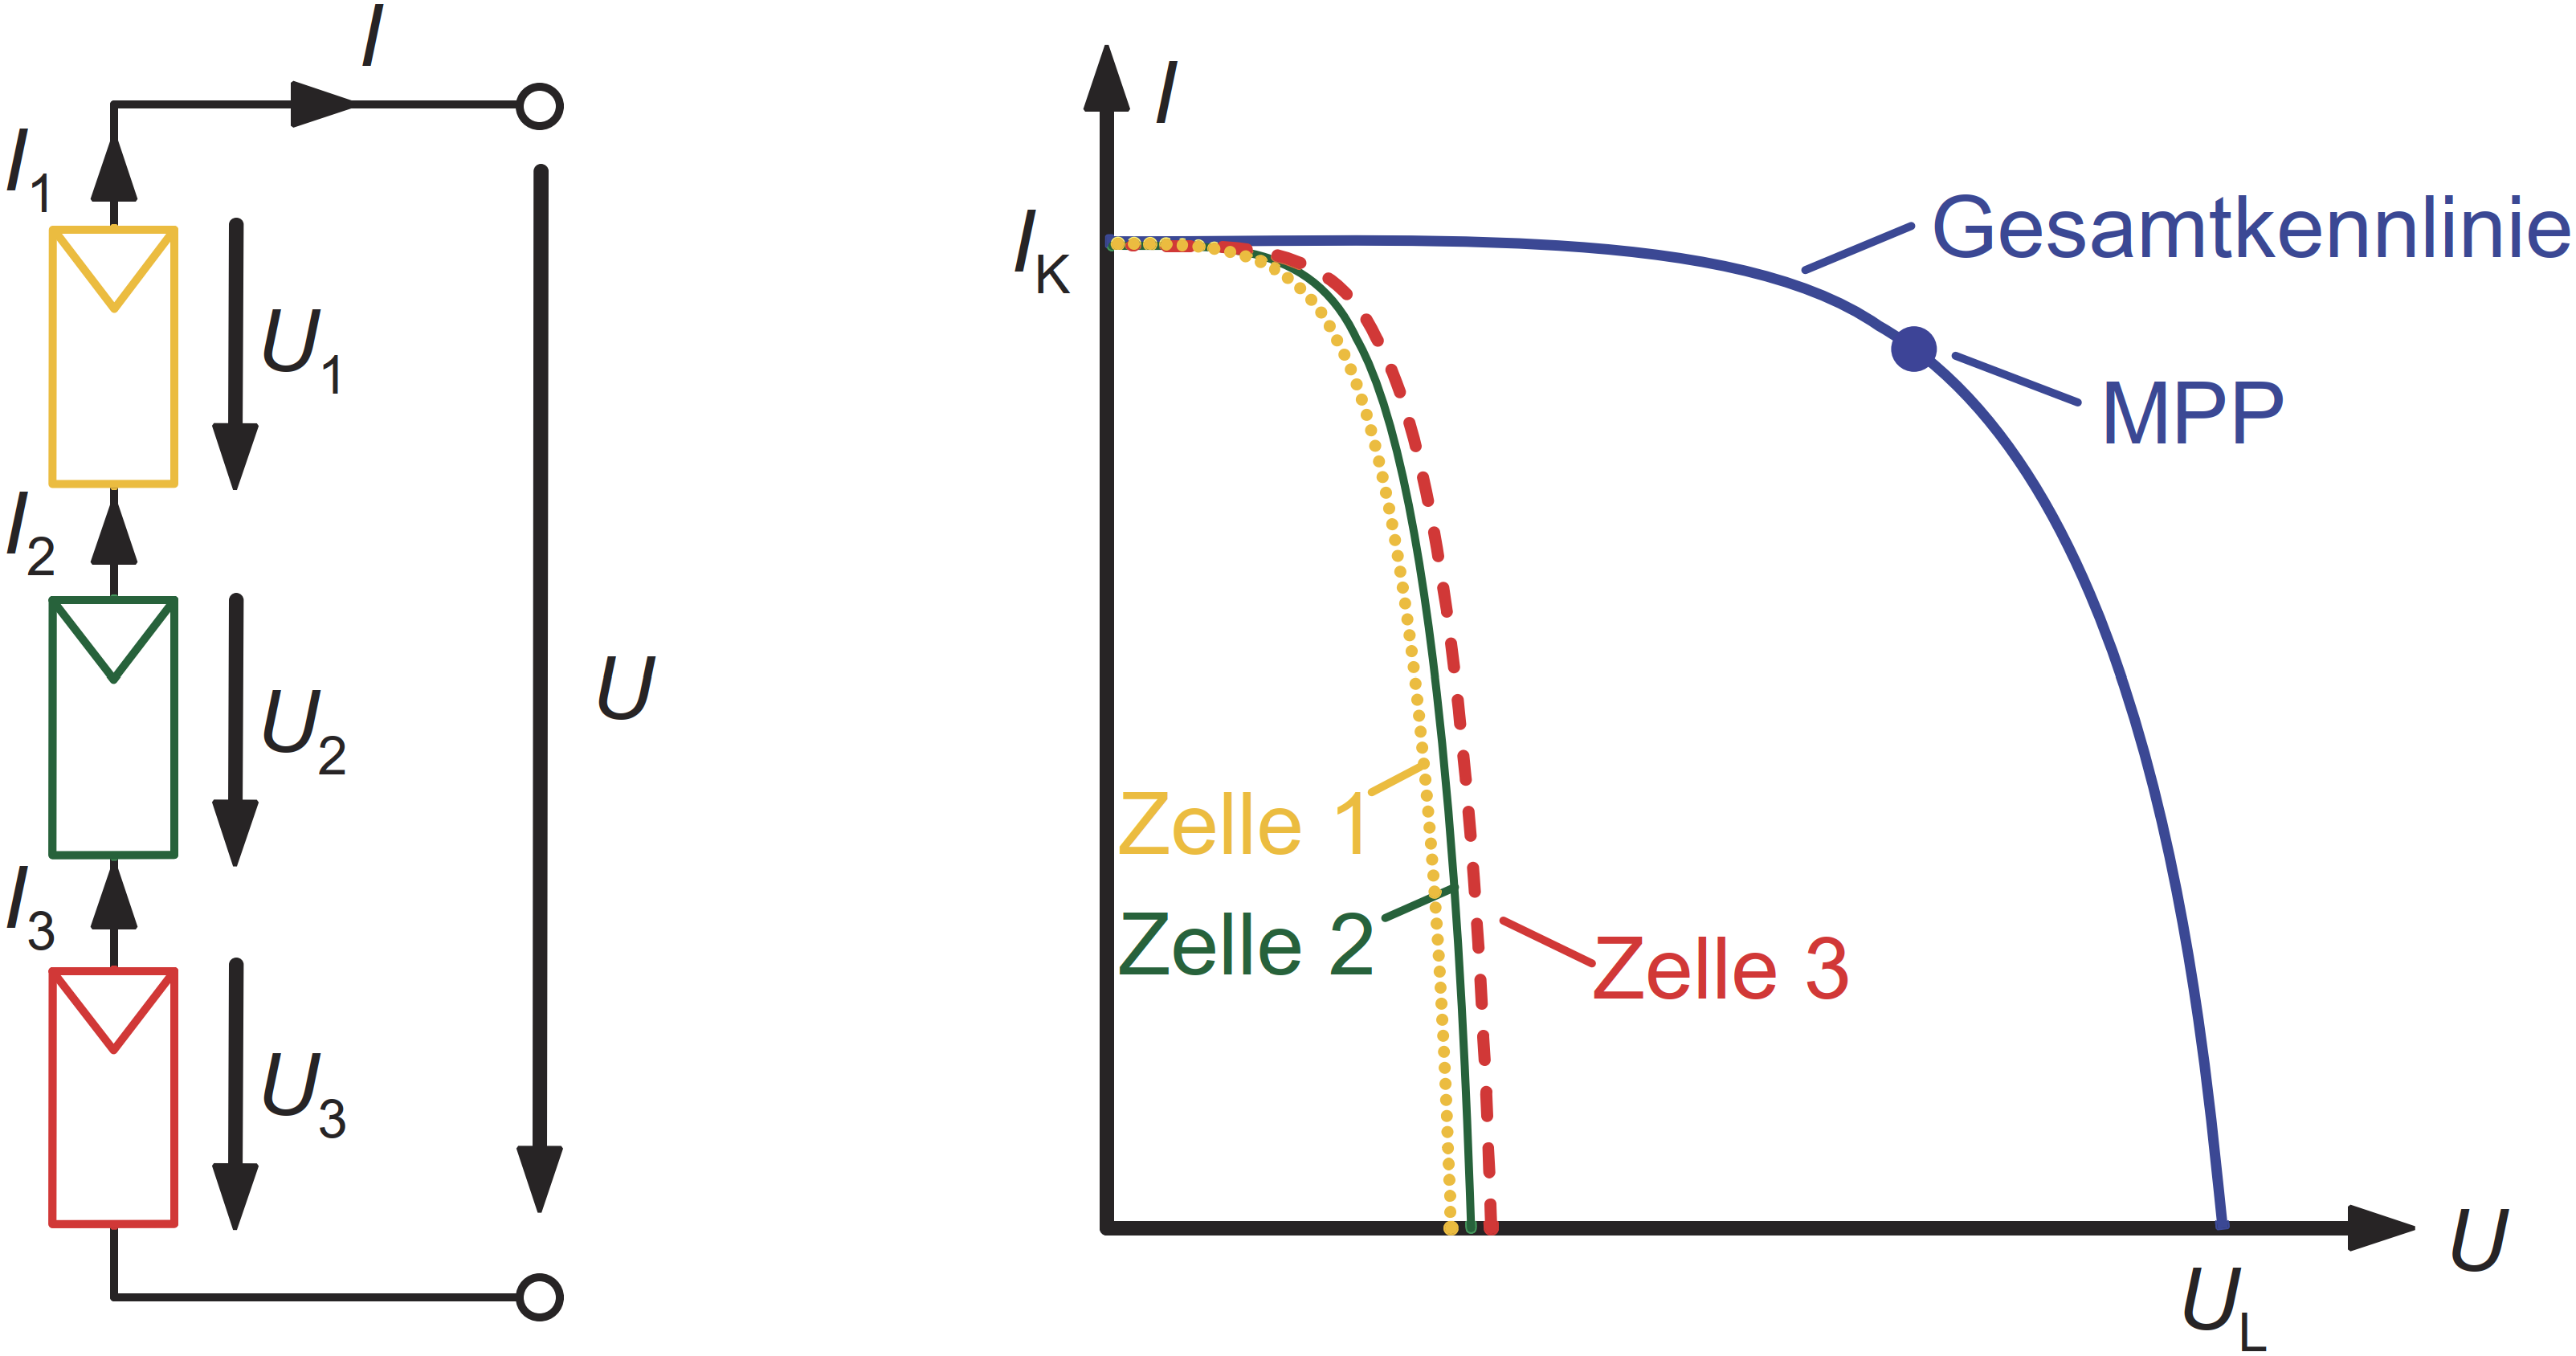
\includegraphics[width=0.95\columnwidth]{images/Serienschaltung_von_Solarzellen.png}


\subsubsection{Serienschaltung mit verschatteter Zelle}
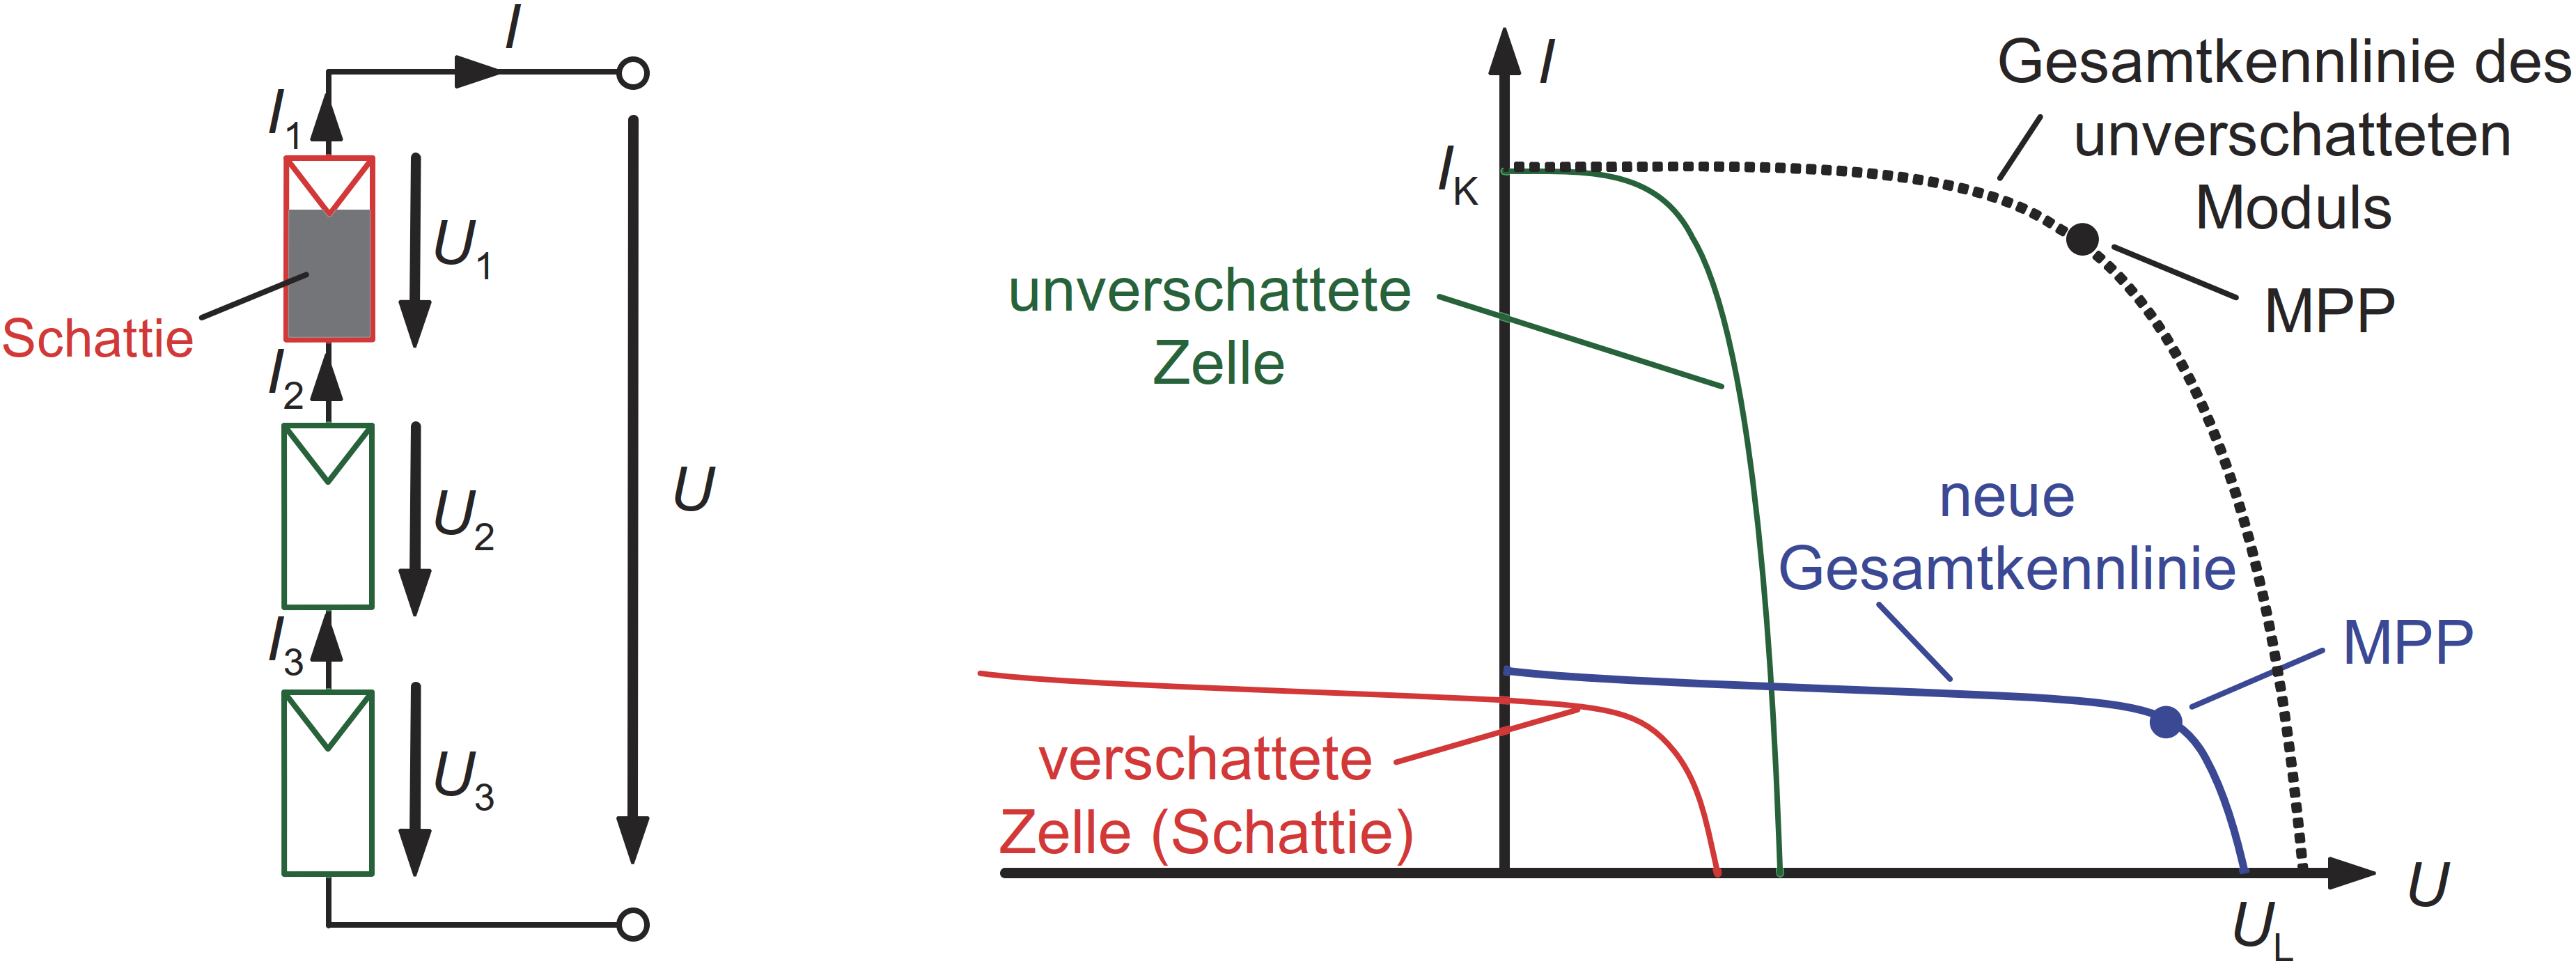
\includegraphics[width=0.95\columnwidth]{images/Serienschaltung_von_Solarzellen_mit_verschatteter_Zelle.png}


\subsection{Parallelschaltung von Solarzellen}
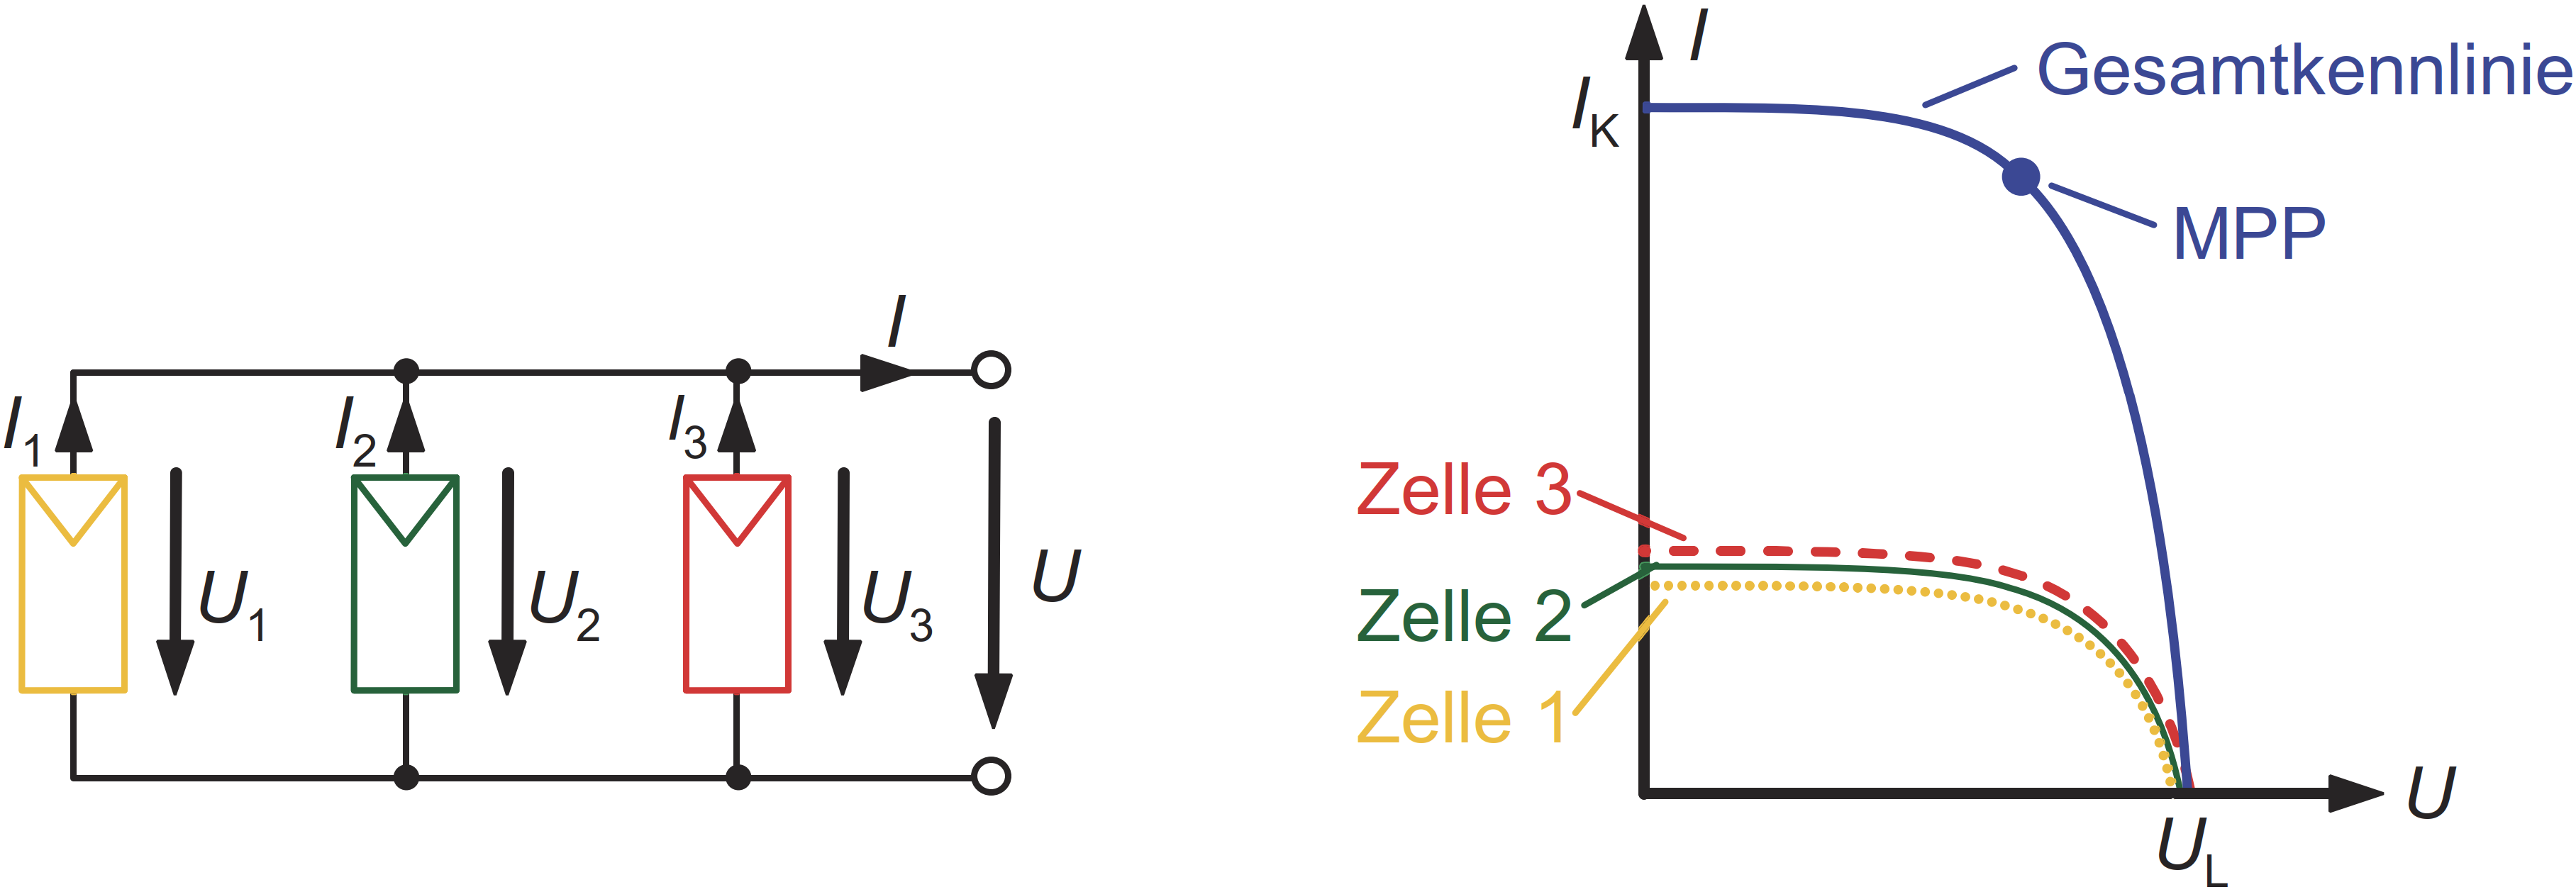
\includegraphics[width=0.95\columnwidth]{images/Parallelschaltung_von_Solarzellen.png}

\subsubsection{Parallelschaltung mit verschatteter Zelle}
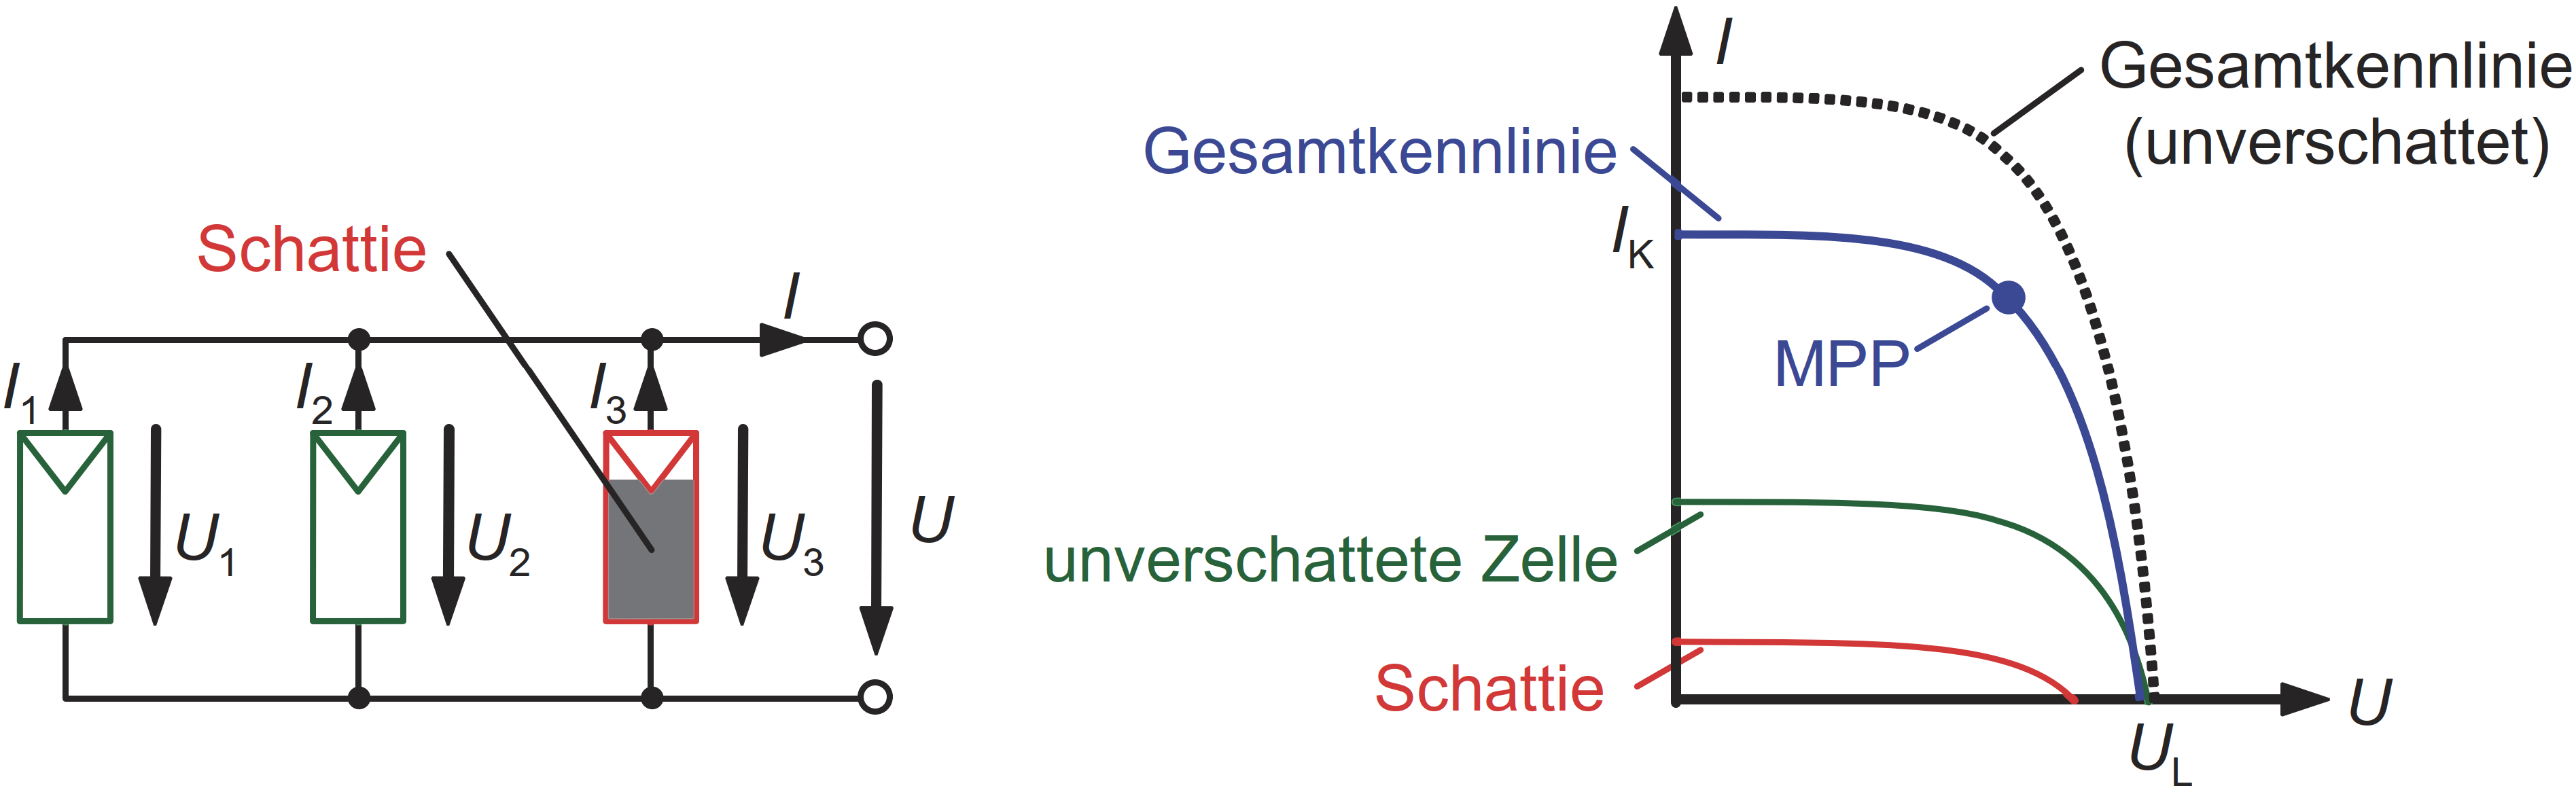
\includegraphics[width=0.95\columnwidth]{images/Parallelschaltung_von_Solarzellen_mit_verschatteter_Zelle.png}

\section{Einsatz von Bypassdioden}
\subsection{Schema Solarmodul}
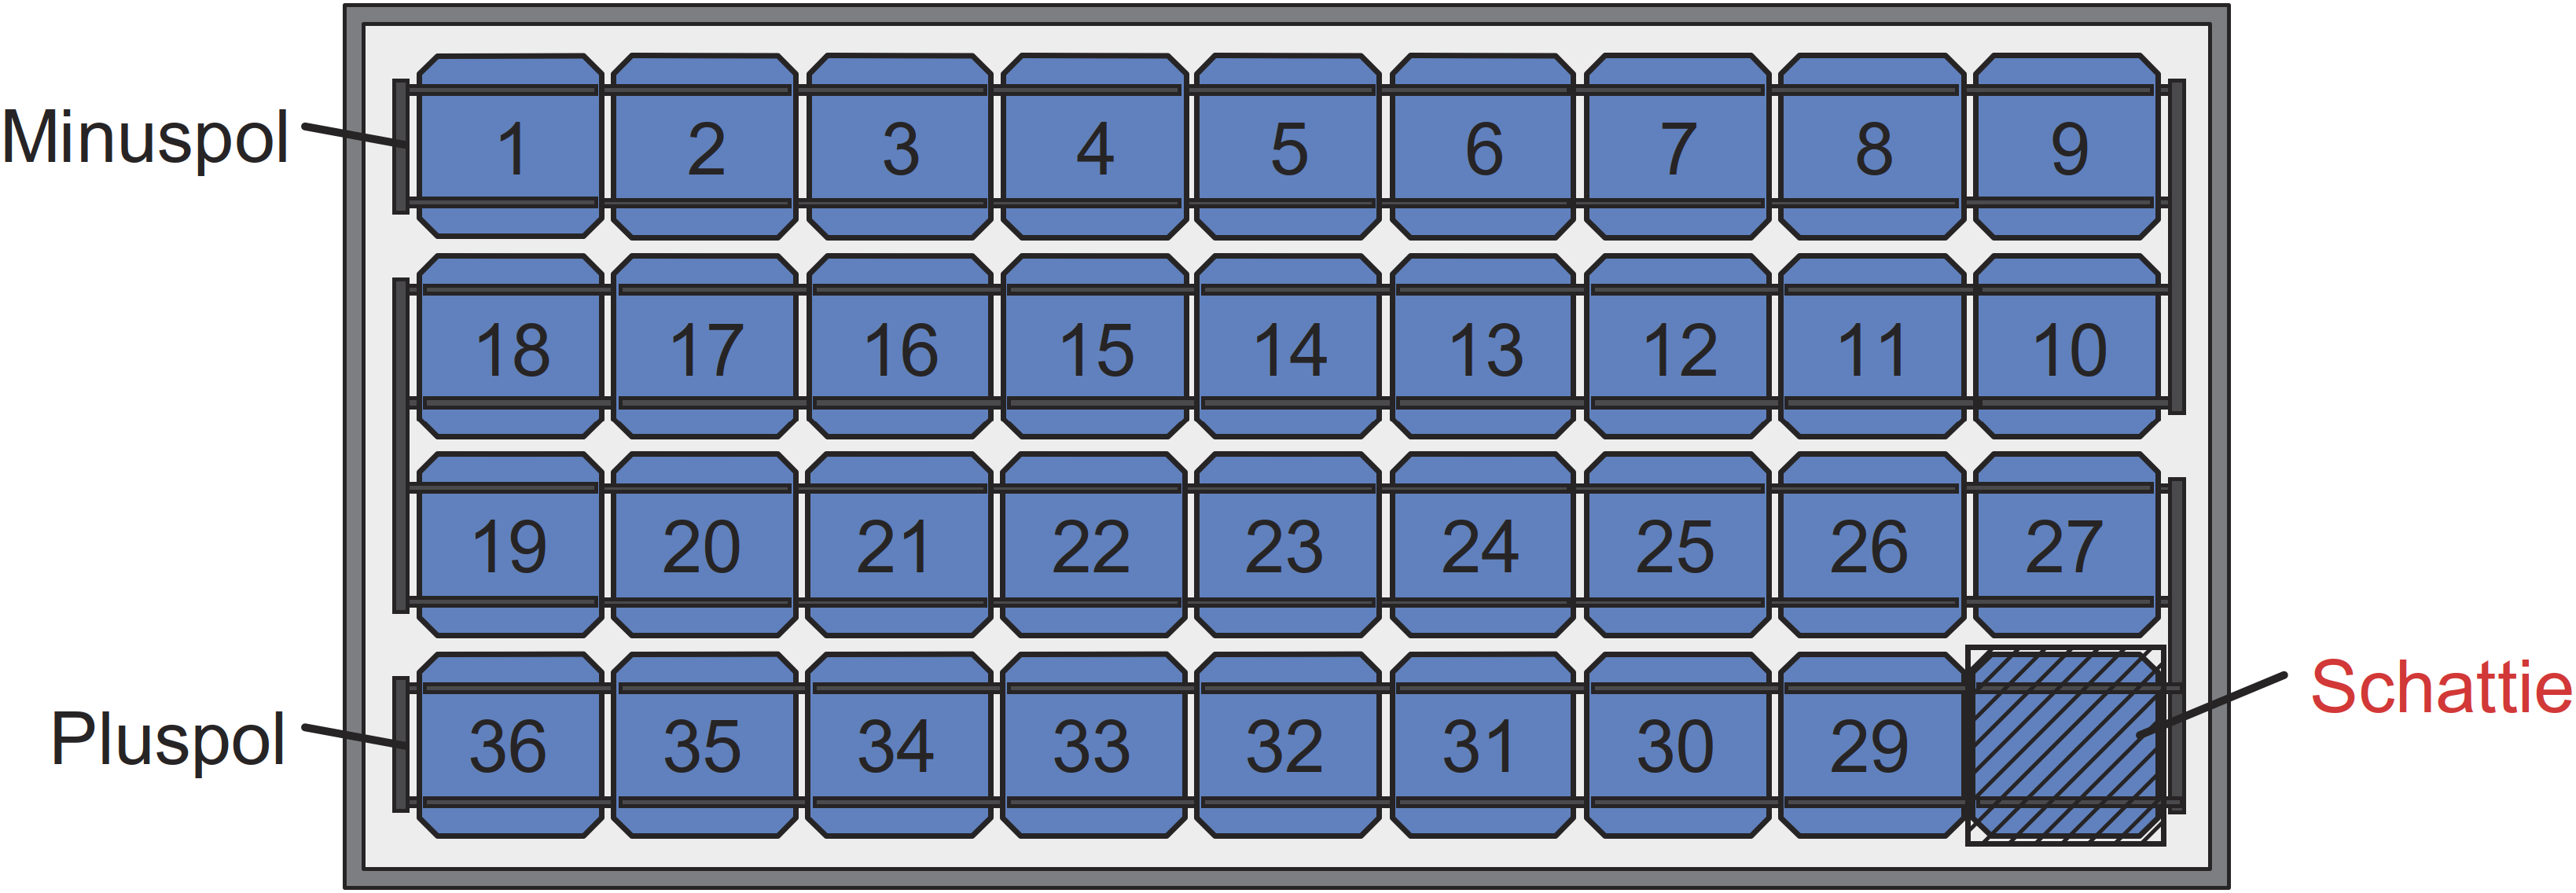
\includegraphics[width=0.95\columnwidth]{images/Verschattungsverluste_Solarmodul.png}

\subsection{Solarmodul ohne Bypassdioden}
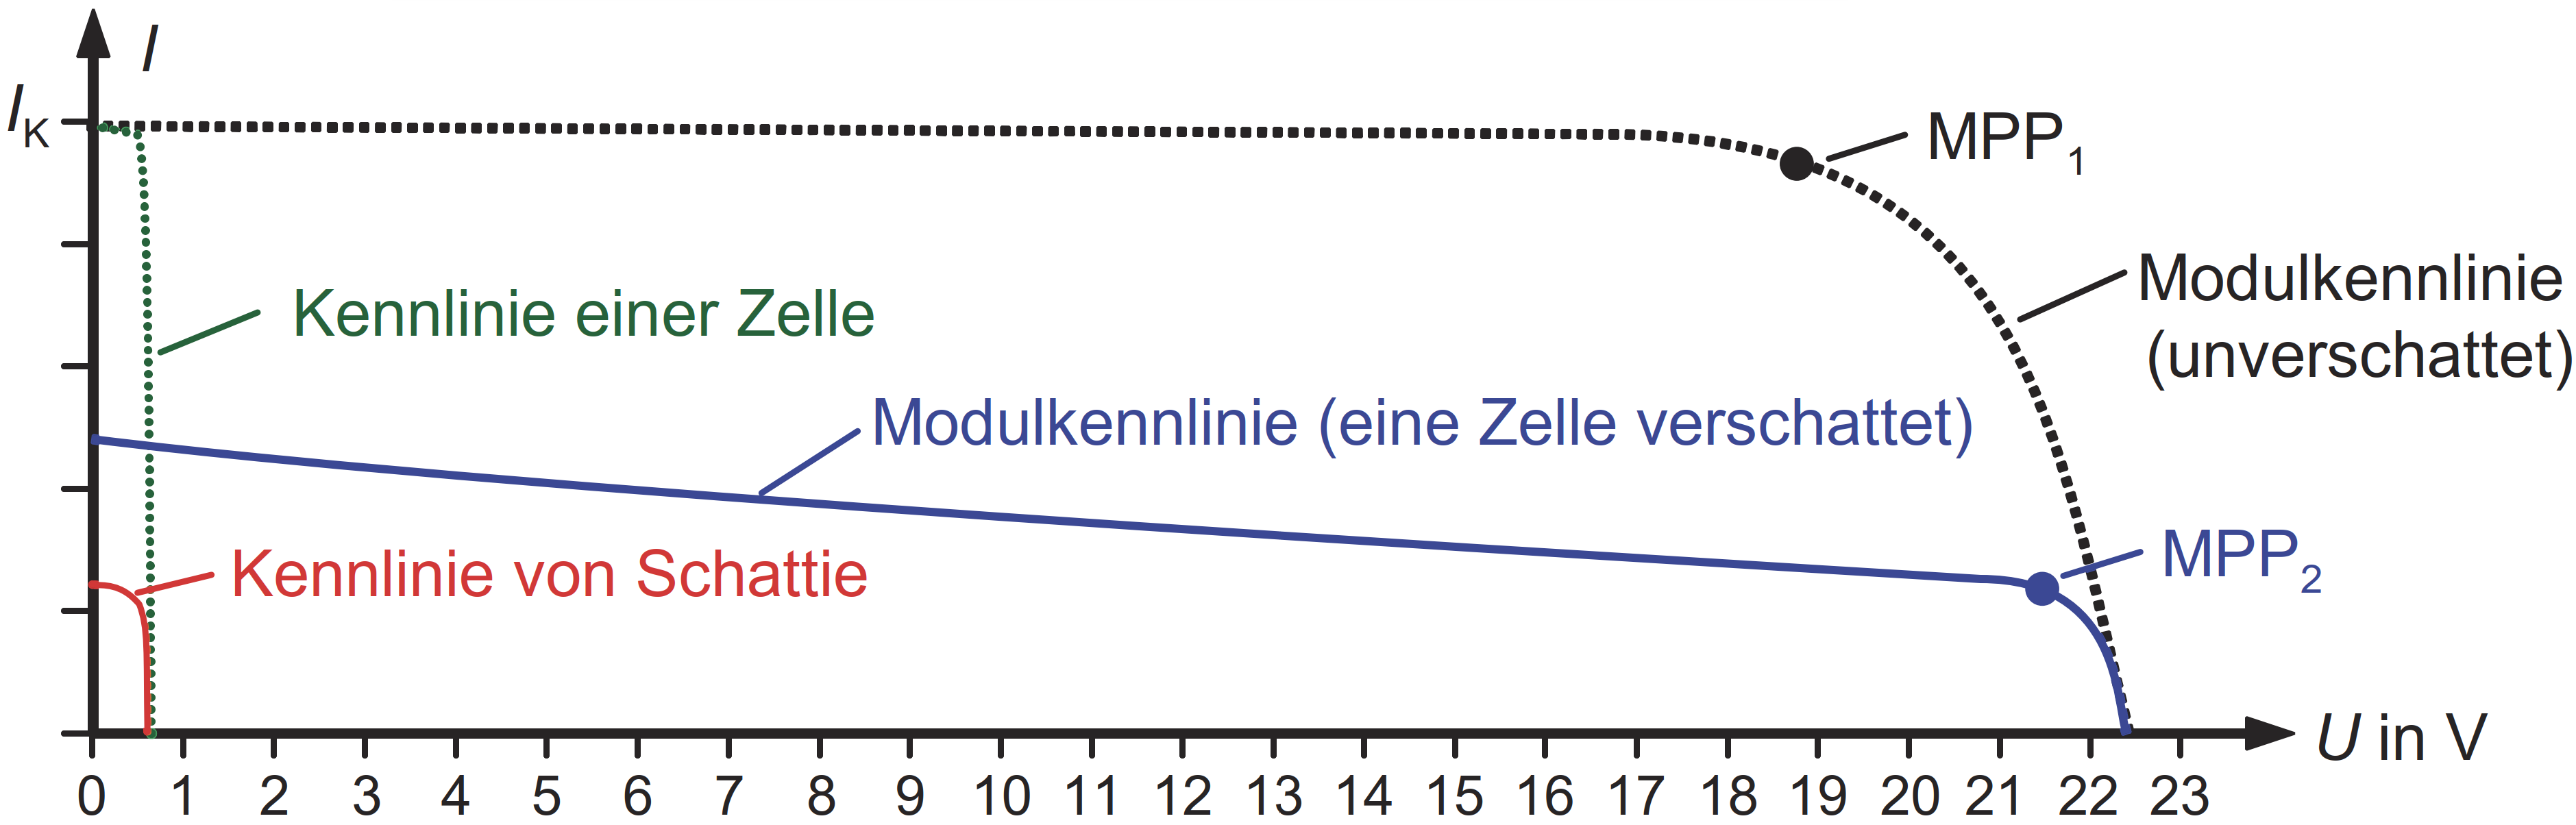
\includegraphics[width=0.95\columnwidth]{images/Verschattungsverluste_ohne_Bypassdiode.png}

\subsection{Solarmodul mit Bypassdioden}
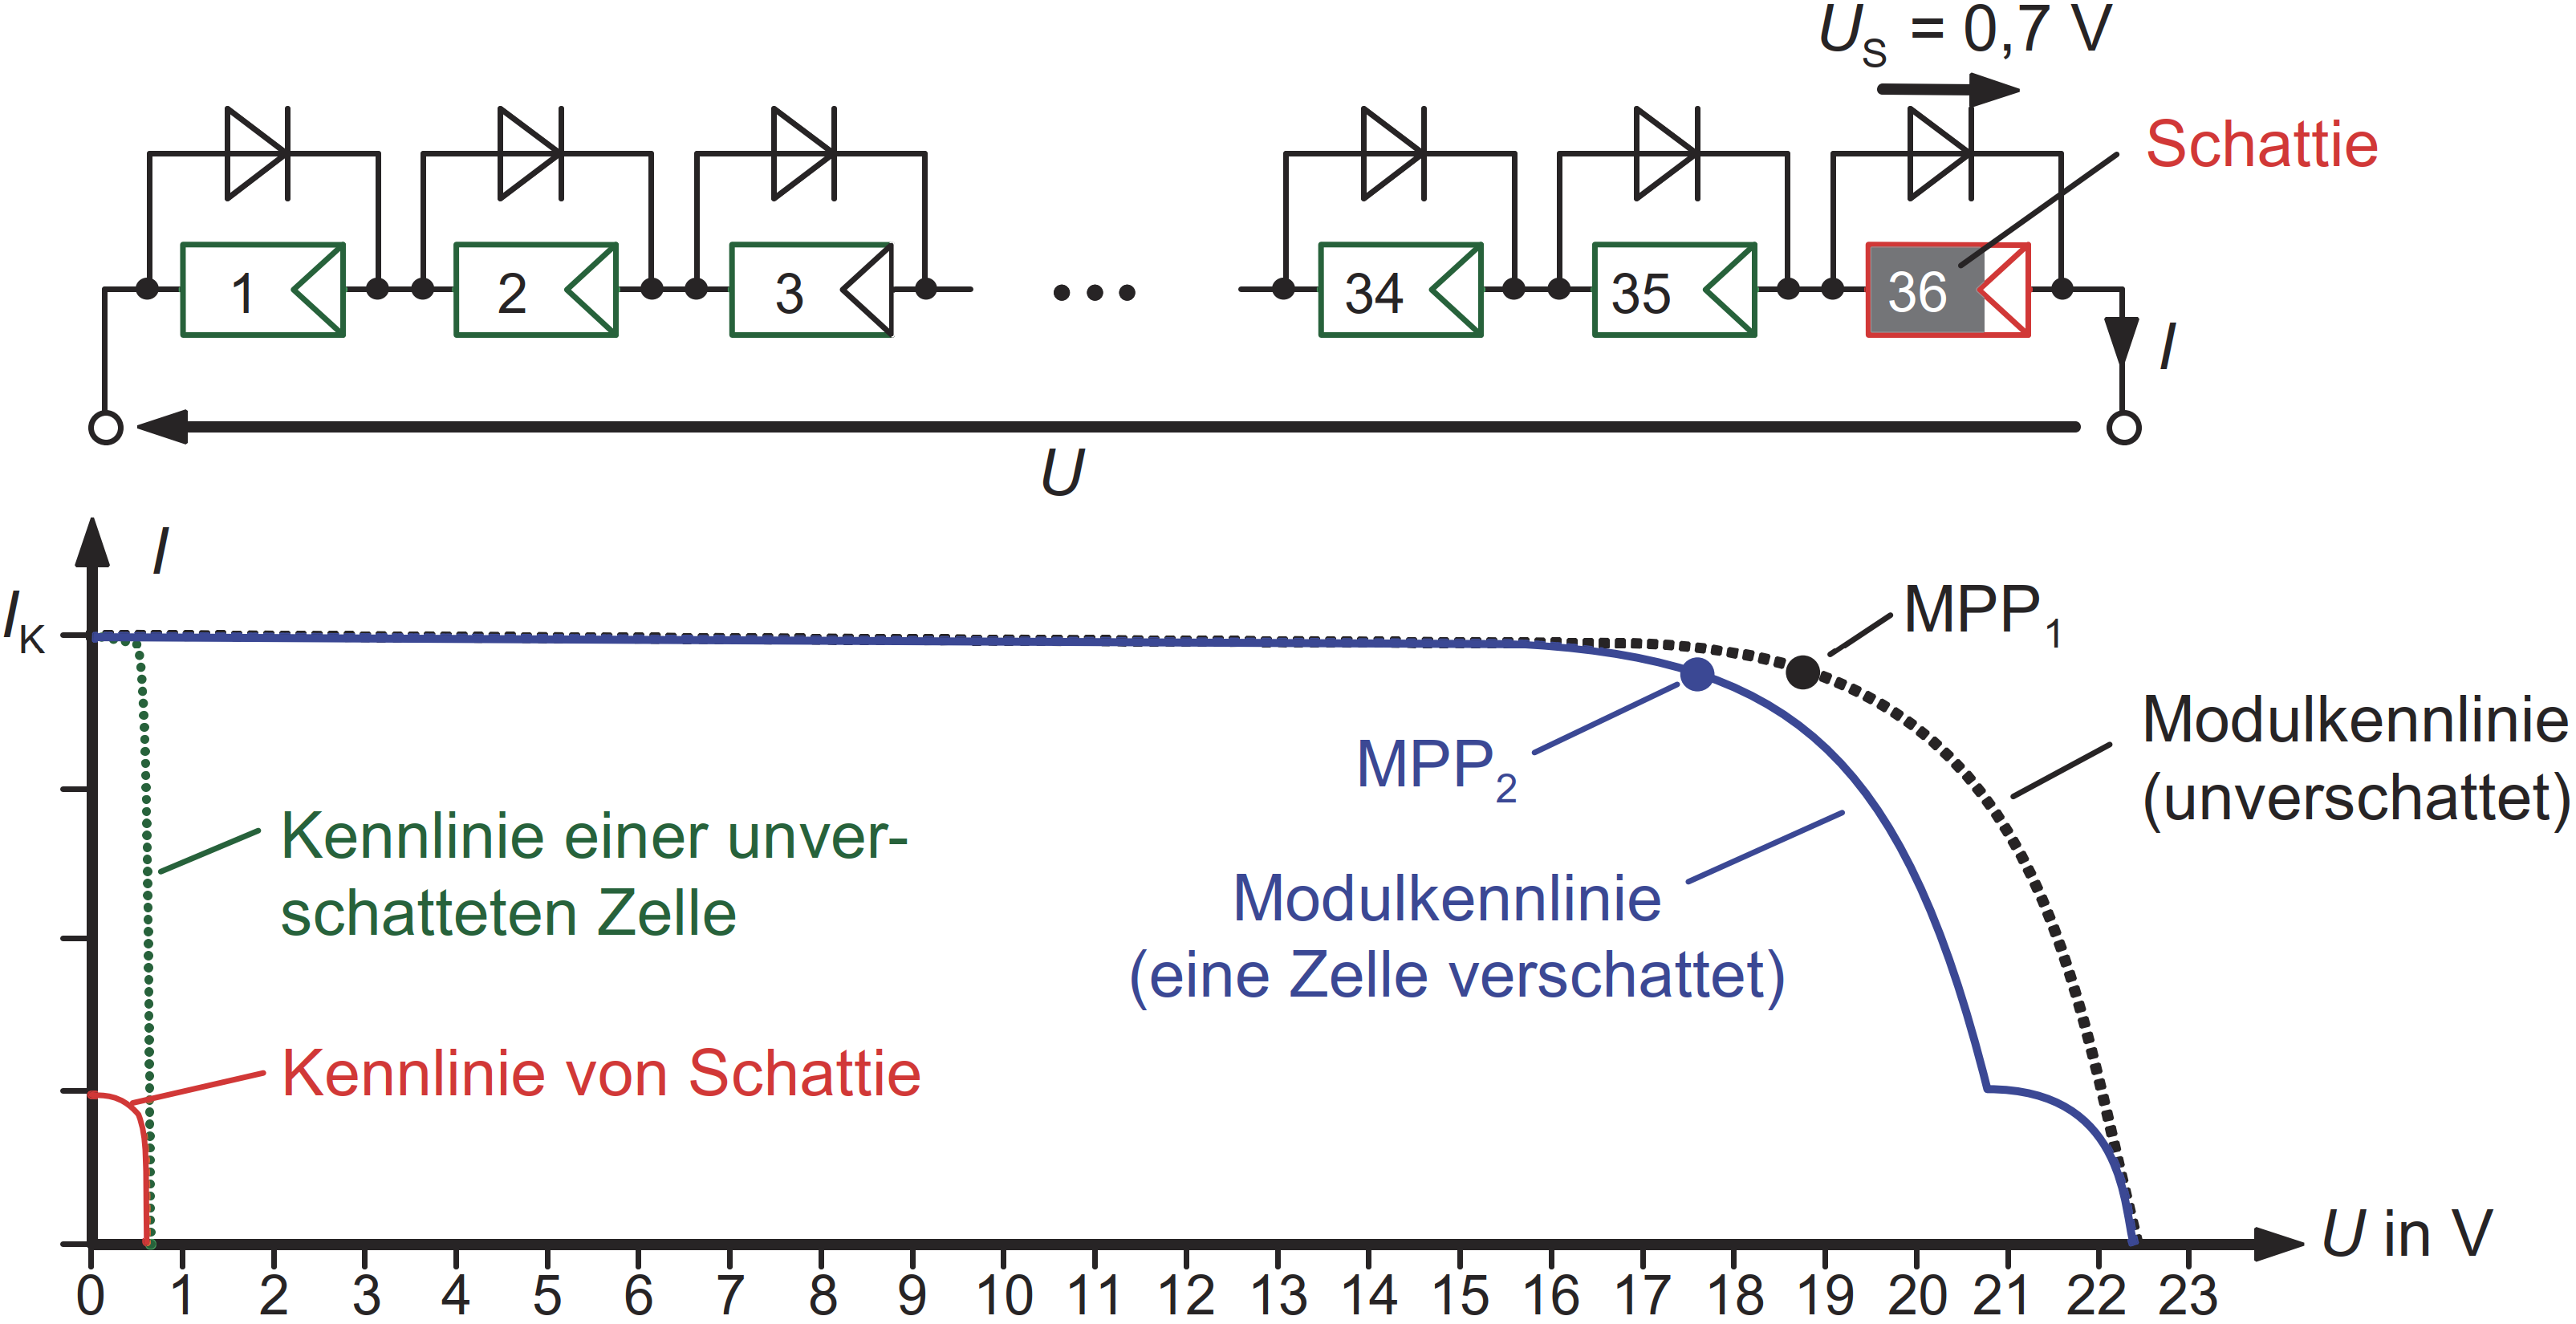
\includegraphics[width=0.95\columnwidth]{images/Verschattungsverluste_mit_Bypassdiode.png}

\subsection{Auswirkung Anzahl Bypassdioden}
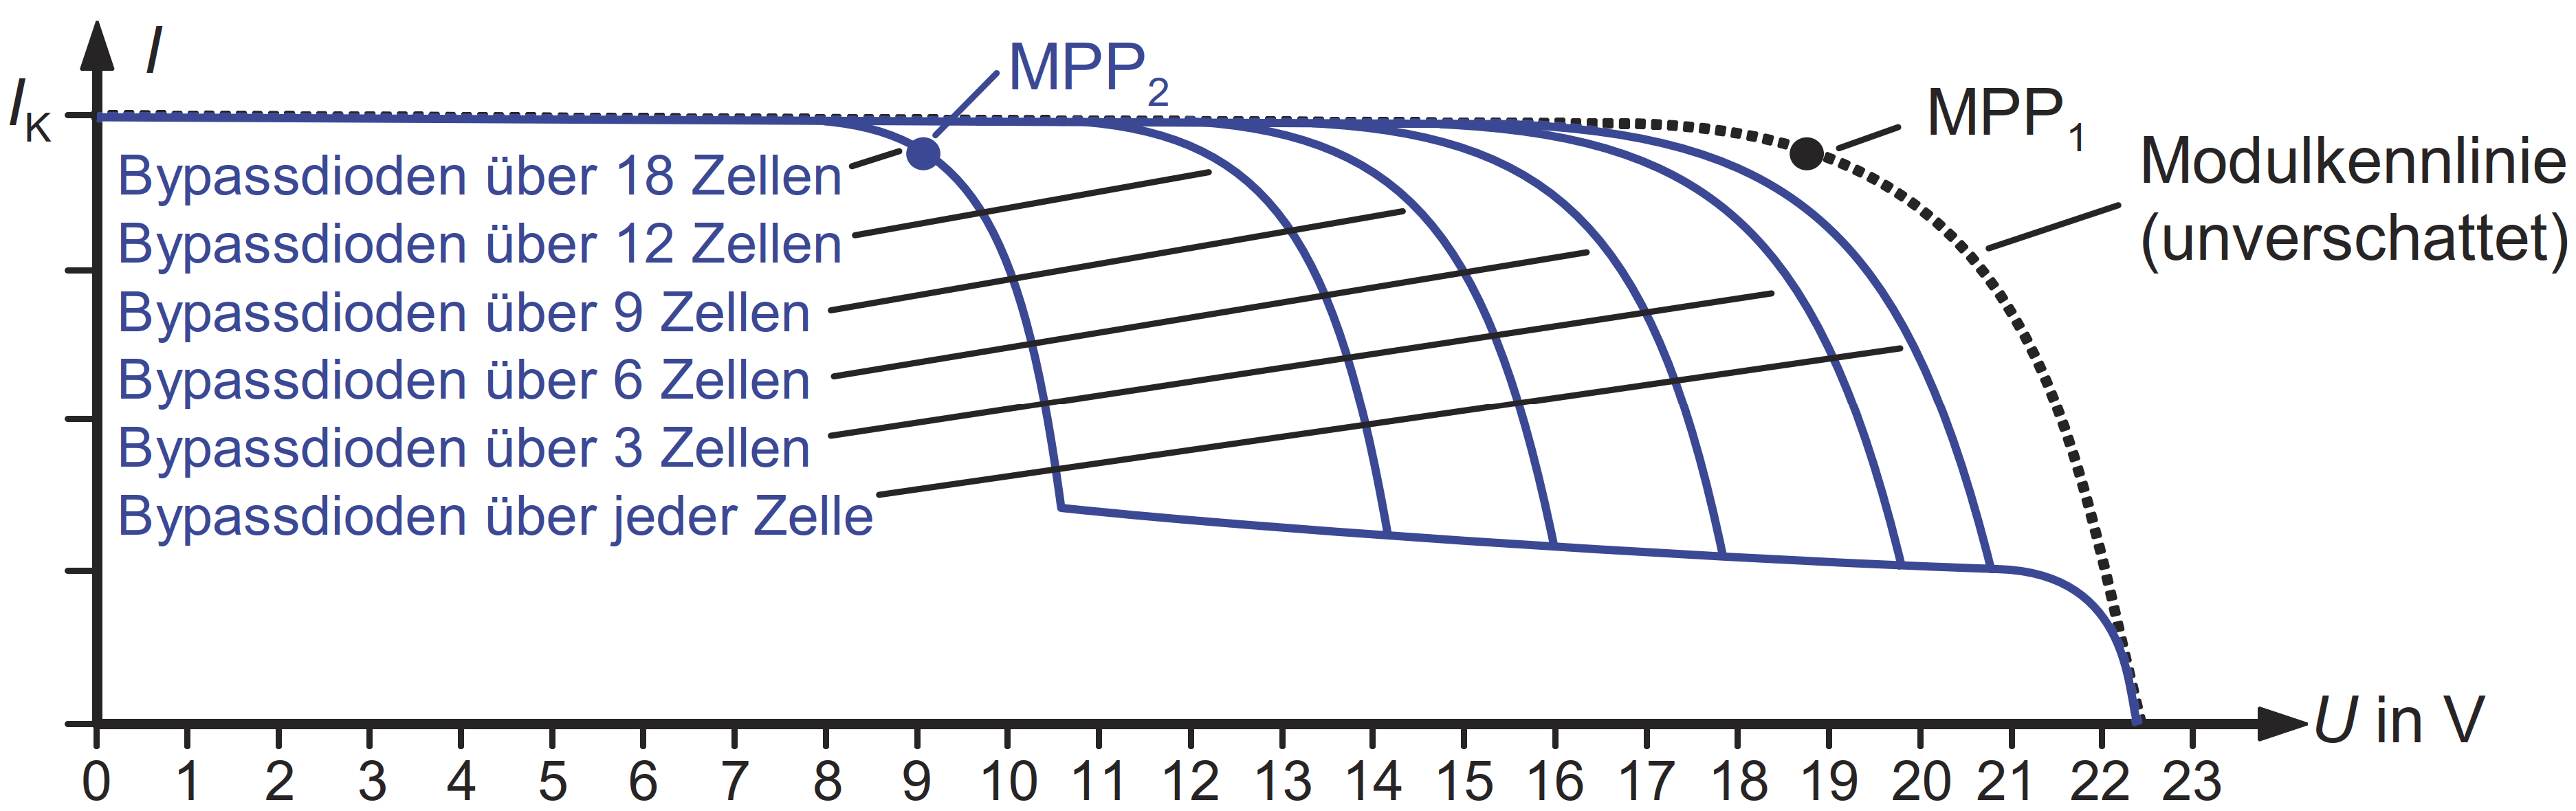
\includegraphics[width=0.95\columnwidth]{images/Reduzierung_Verschattungsverluste_durch_Bypassdioden.png}


\subsection{Vermeidung von Hotspots durch Bypassdioden}
\subsubsection{Solarmodul ohne Bypassdioden}
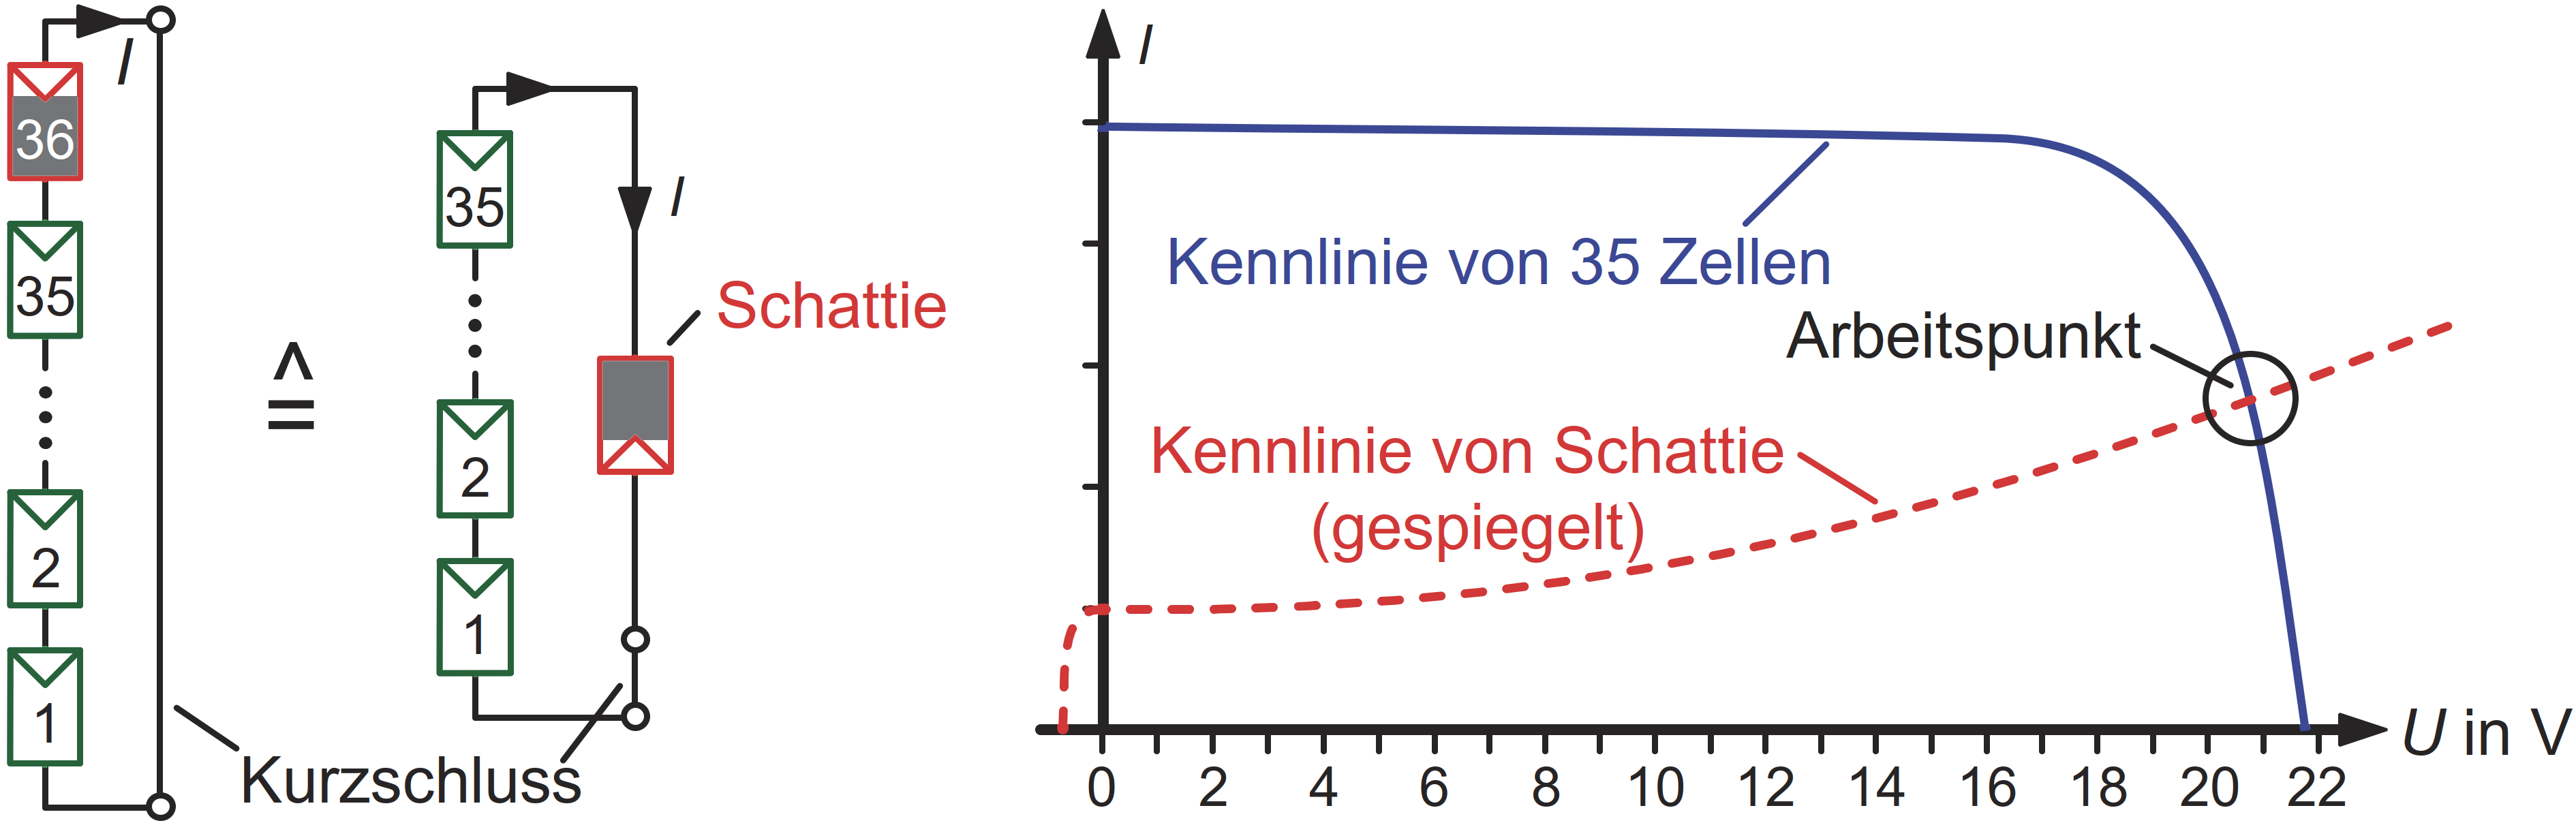
\includegraphics[width=0.95\columnwidth]{images/Vermeidung_von_Hotspots_1.png}

\subsubsection{Solarmodul mit 2 Bypassdioden}
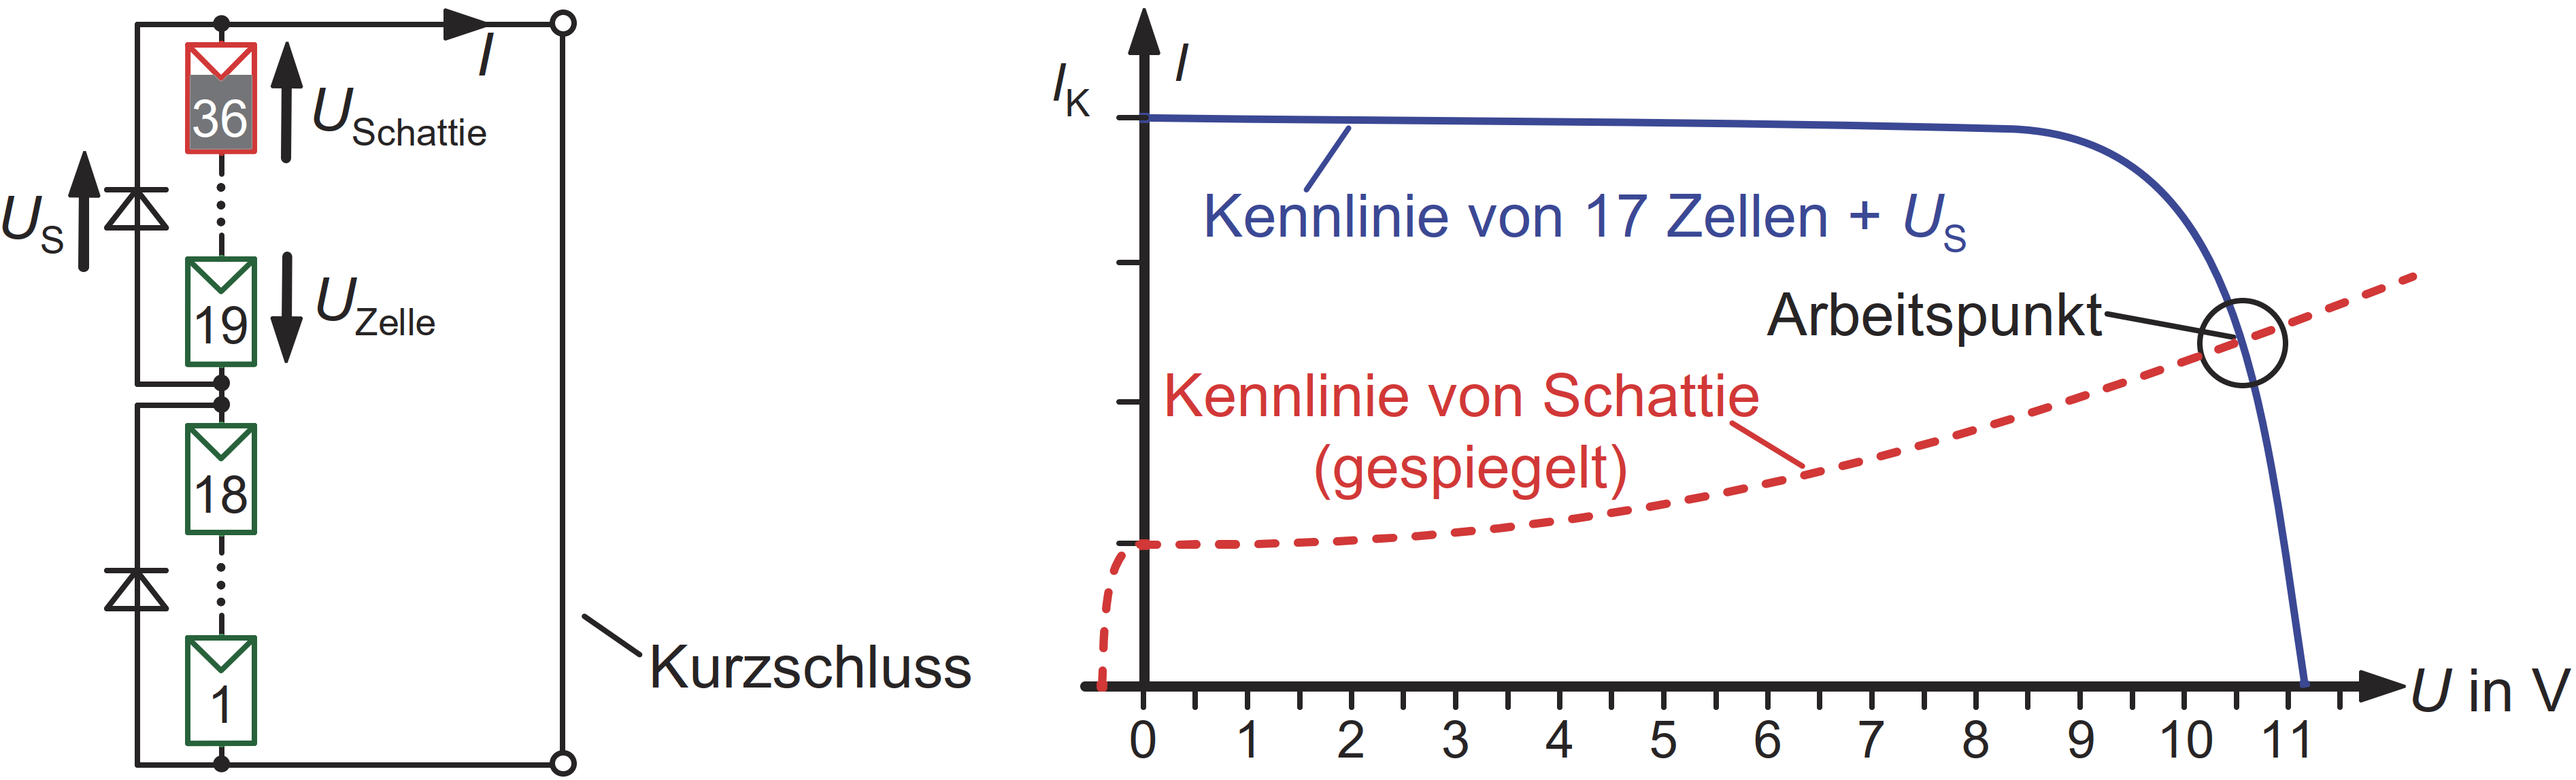
\includegraphics[width=0.95\columnwidth]{images/Vermeidung_von_Hotspots_2.png}

\subsubsection{Betrachtung verschiedener Verschattungsgrade}
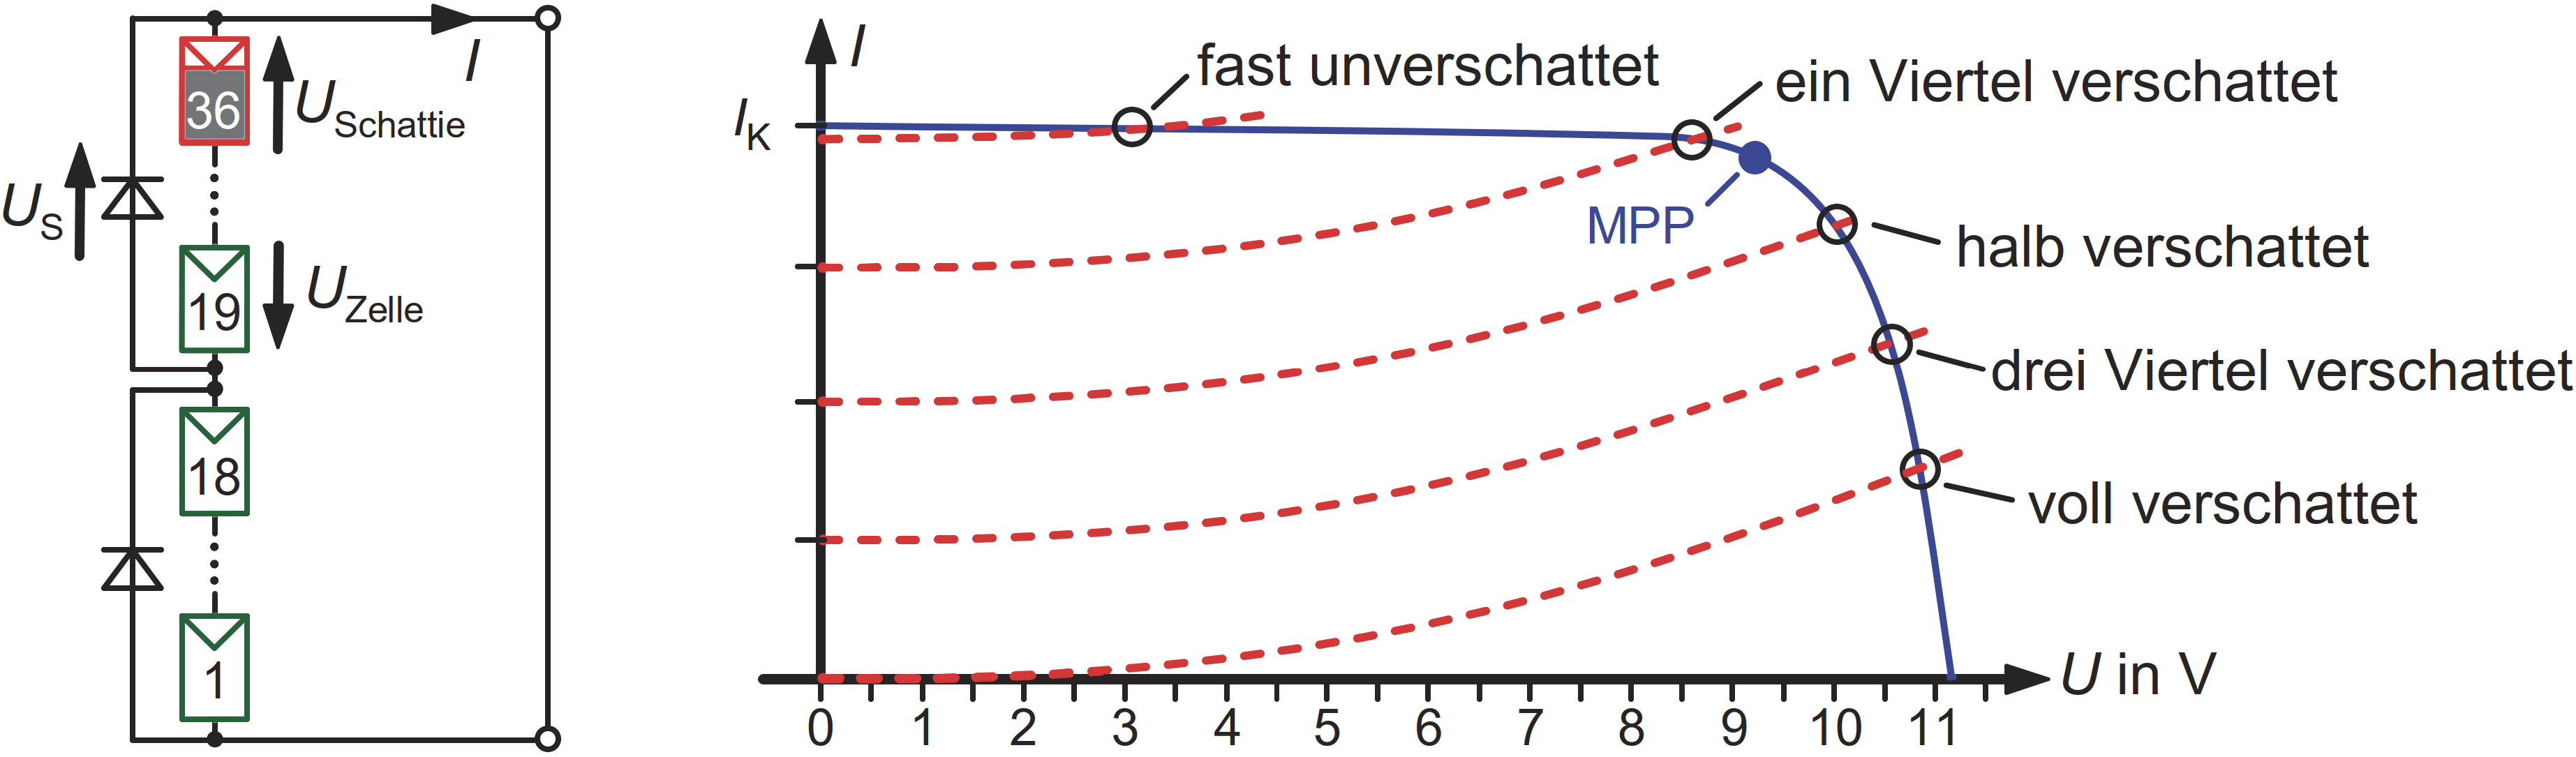
\includegraphics[width=0.95\columnwidth]{images/Vermeidung_von_Hotspots_3.png}

\subsubsection{Keine Hotspots bei Parallelschaltung}
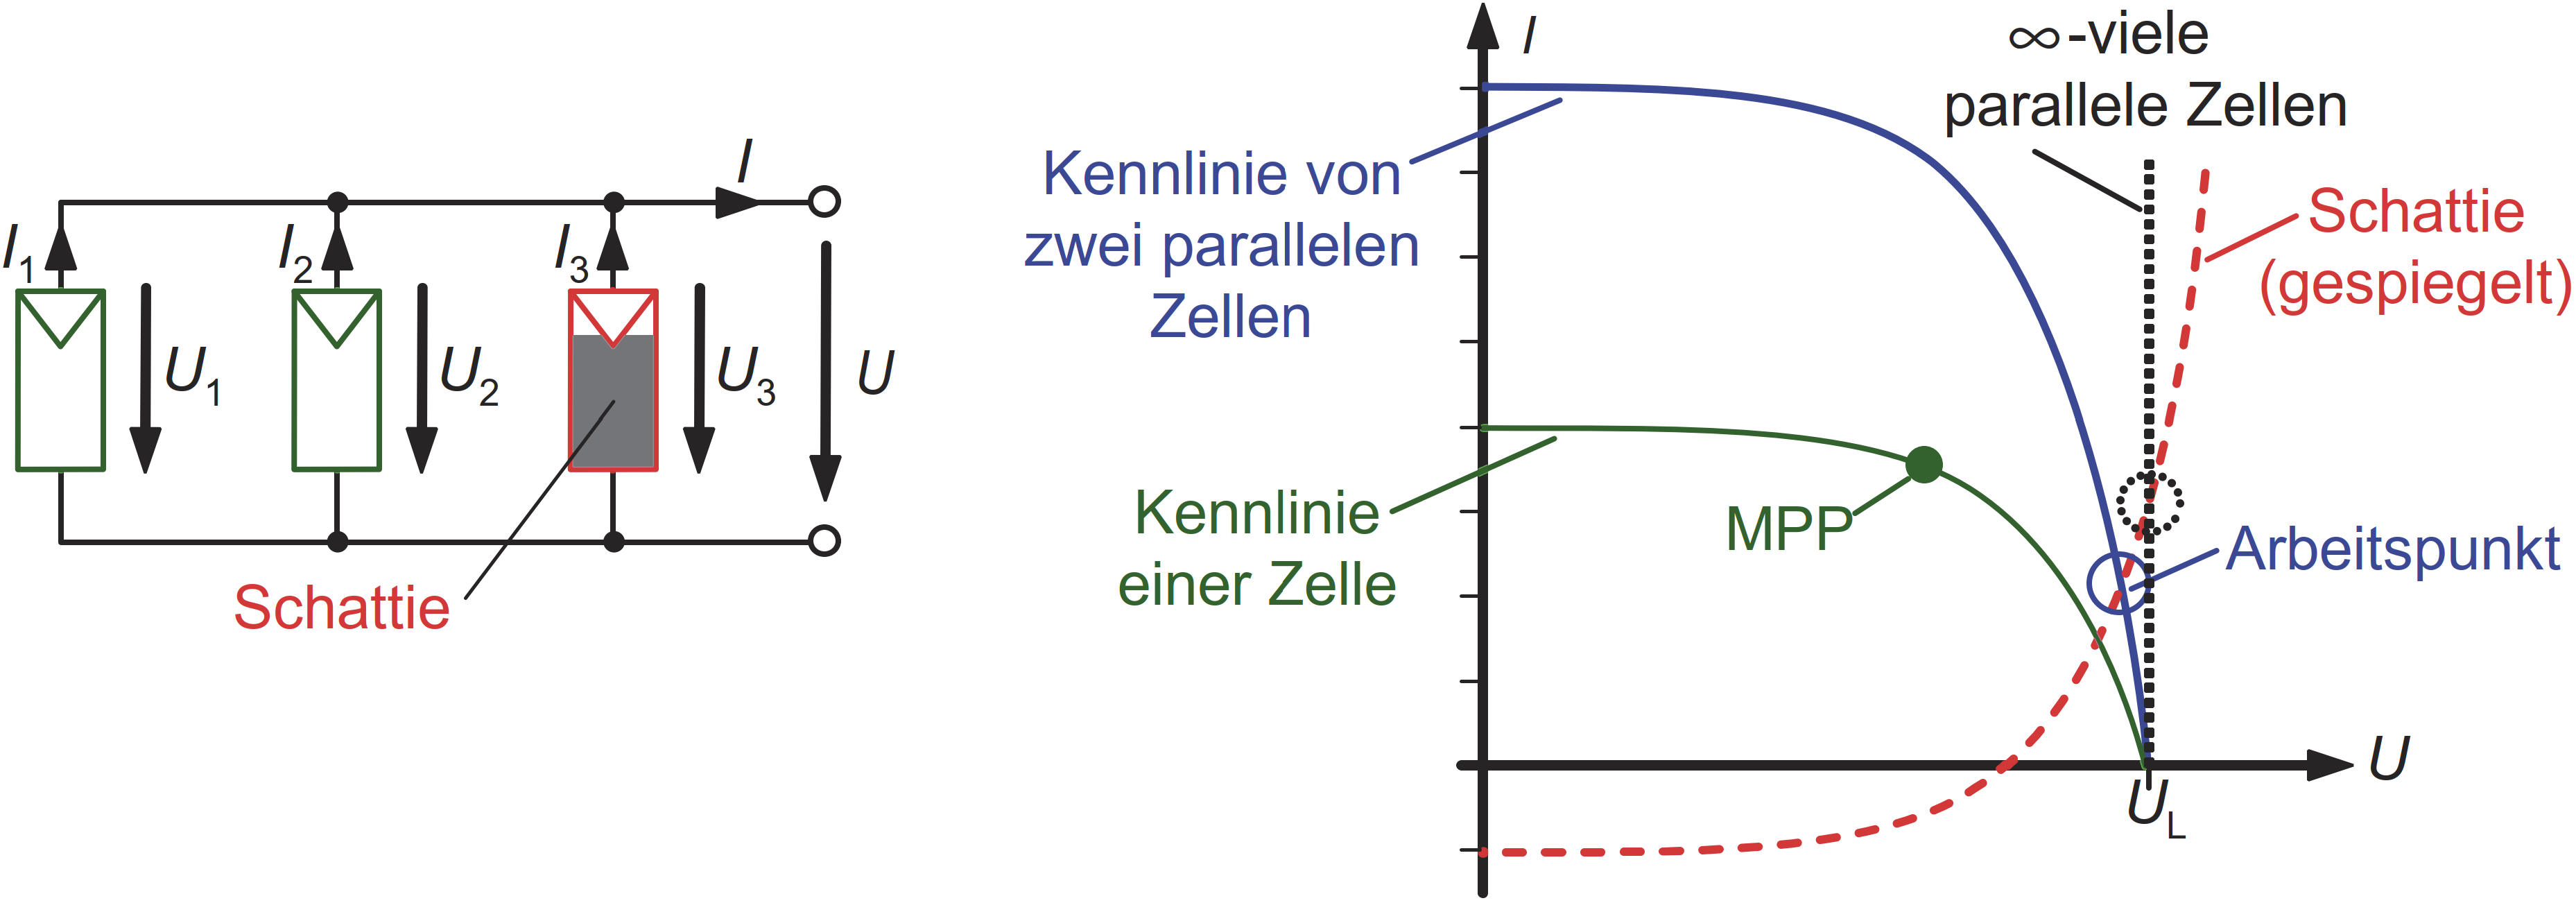
\includegraphics[width=0.95\columnwidth]{images/Keine_Hotspots_bei_Paralellschaltung.png}

\subsection{Bypassdioden bei Voll- und Halbzellenmodulen}

\begin{minipage}[t]{0.48\columnwidth}
    \myul{\textbf{Bypassdioden bei Vollzellenmodulen}}\\
    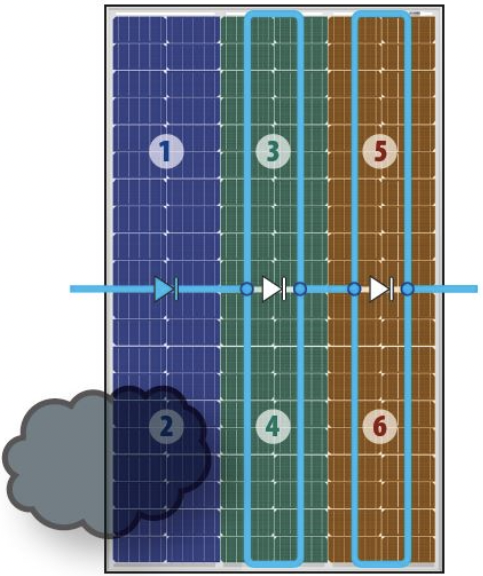
\includegraphics[width=0.9\columnwidth]{images/Bypassdioden bei Vollzellenmodulen.png}
\end{minipage}
\hfill
\begin{minipage}[t]{0.48\columnwidth}
    \myul{\textbf{Bypassdioden bei Halbzellenmodulen}}\\
    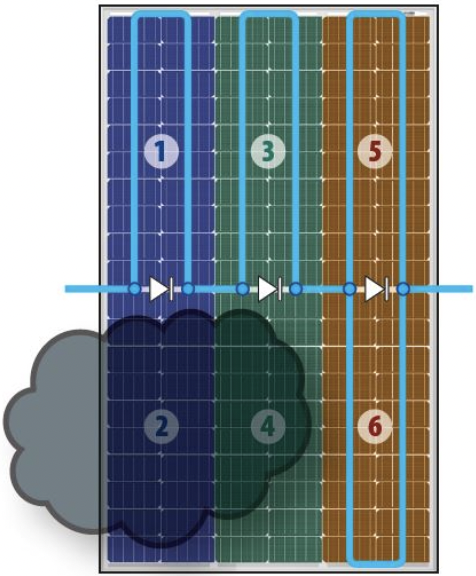
\includegraphics[width=0.9\columnwidth]{images/Bypassdioden bei Halbzellenmodulen.png}
\end{minipage}


\section{Einfluss von Einstrahlung und Temperatur}

\subsection{Standardtestbedingungen (STC - Standard Test Conditions)}
\textbf{Einheitliche Bedingungen für die Bestimmung der Nennleistung von Solarmodulen}

\vspace{0.25cm}

\renewcommand{\arraystretch}{1.5}
\begin{tabular}{|ll|}
    \hline
    Einstrahlung    & $1000\frac{W}{m^2}$ \\
    Zelltemperatur  & $25{^\circ C}$ \\
    Luftmasse AM    & 1.5 \\
    \hline
\end{tabular}

\newcolumn
\subsection{Leistung in Abhängigkeit von Einstrahlung und Temperatur}

Die Leistung $P_{MPP}$ am Maximum Power Point (MPP) einer Solarzelle berechnet sich nach folgender Formel:

$
\boxed{
P_{MPP} = P_{STC} \cdot \frac{G}{G_{STC}} \cdot \left[1 + \alpha_P \cdot (\vartheta_{\text{Zell}} - \vartheta_{\text{Zell,STC}}) \right]
}
$

\vspace{0.25cm}

\renewcommand{\arraystretch}{1.2} % Erhöht Zeilenhöhe für bessere Lesbarkeit
\begin{tabular}{@{} l p {6cm} l @{}}
    $[P_{MPP}]$       & Leistung im Maximum Power Point \dotfill & $W$ \\
    $[P_{STC}]$       & Leistung bei Standardtestbedingungen \dotfill & $W$ \\
    $[G]$             & Globalstrahlung \dotfill & $\frac{W}{m^2}$ \\
    $[G_{STC}]$       & Globalstrahlung bei STC = 1000 W/m² \dotfill & $\frac{W}{m^2}$ \\
    $[\alpha_P]$      & Temperaturkoeffizient der Leistung \dotfill & $\frac{\%}{^\circ C}$ \\
    $[\vartheta_{\text{Zell}}]$ & Zelltemperatur \dotfill & $^\circ C$ \\
    $[\vartheta_{\text{Zell,STC}}]$ & Zelltemperatur bei STC = 25°C \dotfill & $^\circ C$ \\
\end{tabular}


\subsection{Strom und Spannung (Einstrahlung und Temperatur)}

Die Abhängigkeit von Strom und Spannung einer Solarzelle von der Einstrahlung und Temperatur wird durch folgende Gleichungen beschrieben:

$
\boxed{
I_K = I_{K,STC} \cdot \frac{G}{G_{STC}} \cdot \left[1 + \alpha_I \cdot (\vartheta_{\text{Zell}} - \vartheta_{\text{Zell,STC}}) \right]
}
$

$
\boxed{
U_L = U_{L,\text{Grafik}} \cdot \left[1 + \alpha_U \cdot (\vartheta_{\text{Zell}} - \vartheta_{\text{Zell,STC}}) \right]
}
$

$
\boxed{
I_{MPP} = I_{MPP,STC} \cdot \frac{G}{G_{STC}} \cdot \left[1 + \alpha_I \cdot (\vartheta_{\text{Zell}} - \vartheta_{\text{Zell,STC}}) \right]
}
$

$
\boxed{
U_{MPP} = \frac{P_{MPP}}{I_{MPP}}
}
$

\vspace{0.25cm}

\renewcommand{\arraystretch}{1.2} % Erhöht Zeilenhöhe für bessere Lesbarkeit
\begin{tabular}{@{} l p {7cm} l @{}}
    $[I_K]$         & Kurzschlussstrom (G, $\vartheta_{\text{Zell}}$) \dotfill & $A$ \\
    $[I_{K,STC}]$   & Kurzschlussstrom bei Standardtestbedingungen \dotfill & $A$ \\
    $[U_L]$         & Leerlaufspannung (G, $\vartheta_{\text{Zell}}$) \dotfill & $V$ \\
    $[U_{L,\text{Grafik}}]$ & Leerlaufspannung (G) aus Grafik \dotfill & $V$ \\
    $[I_{MPP}]$     & Strom im Maximum Power Point (G, $\vartheta_{\text{Zell}}$) \dotfill & $A$ \\
    $[I_{MPP,STC}]$ & Strom im Maximum Power Point bei STC \dotfill & $A$ \\
    $[U_{MPP}]$     & Spannung im Maximum Power Point (G, $\vartheta_{\text{Zell}}$) \dotfill & $V$ \\
    $[G]$           & Globalstrahlung \dotfill & $\frac{W}{m^2}$ \\
    $[G_{STC}]$     & Globalstrahlung bei STC = 1000 W/m² \dotfill & $\frac{W}{m^2}$ \\
    $[\alpha_I]$    & Temperaturkoeffizient des Kurzschlussstroms \dotfill & $\frac{\%}{^\circ C}$ \\
    $[\alpha_U]$    & Temperaturkoeffizient der Leerlaufspannung \dotfill & $\frac{\%}{^\circ C}$ \\
    $[\vartheta_{\text{Zell}}]$ & Zelltemperatur \dotfill & $^\circ C$ \\
    $[\vartheta_{\text{Zell,STC}}]$ & Zelltemperatur bei STC = 25°C \dotfill & $^\circ C$ \\
\end{tabular}









